% Latex

- comentários de uma linha com: %
- o ficheiro contém o texto do documento assim como os comandos que dizem ao L A TEX como formatar o texto.
- Caracteres “brancos” como espaços ou caracteres de tabulação (tabs) são tratados uniformemente como “espaços” pelo LATEX.
- Caracteres brancos consecutivos são tratados como um “espaço”.
- Espaços no inicio da linha são ignorados
- Quebra de linha é lida como espaço
- Uma ou muitas linhas vazias entre 2 linhas de texto marcam o fim de um parágrafo
- chaves {} são usadas para delimitar comandos
- A barra dupla \\ é uma quebra de linha
- tem que instalar os arquivos para português do babel: sudo apt-get install texlive-lang-portuguese


% Arquivo .tex:
O arquivo .tex é dividido em:
	Preâmbulo		: contém informações globais - tipo de texto, imagens, fontes
	Corpo do texto	: texto propriamente dito
	
%Exemplo de arquivo .tex:
	%isto é o preambulo, article é o nome da classe, entre []s são as opçoes
	\documentclass[a4paper, 12pt]{article}		

	%para cada \begin haverá um \end correspondente
	\begin{document}	
	 O texto vem aqui
	\end{document}


%____________________________________________________________________________


% Comandos

- a classe article tem formatações pré estabelecidas como margens e numeração de página
- linhas em branco = 1 parágrafo
- notações matemáticas: $ax^2 + bx + c = 0$
- notações matemáticas quebrando linha e centralizando: $$ax^2 + bx + c = 0$$

%%% Constantes
\pi

%%% Símbolos matemáticos
\neq 			%not equal
\overline{AB}	%linha sobre AB = segmento AB


%%% Caracteres especiais (outros:  $  ^ & _ { } ~ \ # $)
\c c == ç 
\~a == ã
\'o == ó
\^o == ô
2$^\circ$ == 2°

%%% Formatações de texto:
\begin{center}
	Texto centraliazado, outras opções: flushright, flushleft
\end{center}

\textbf{texto em negrito}
\textit{texto em itálico}
\underline{texto sublinhado}

%%% programas
texmaker	www.xm1math.net/texmaker/
texlive  	www.tug.org/texlive/

%%% Texmaker é um editor LaTeX open source com um visualizador de PDF integrado.
	Atalhos
	F6 = Gera PDF
	F7 = Ver PDF


%%% links 

	





%____________________________________________________________________________

%Exemplo báskhara: (ver no programa TexMaker):

\documentclass[a4paper, 12pt]{article}									%classe article com opções papel A4 e fonte 12pt
\usepackage[top=2cm, bottom=2cm, left=2.5cm, right=2.5cm]{geometry}		%pacote geometry para margens do texto
\usepackage[utf8]{inputenc}												%pacote inputenc para identificar caract especiais 
\begin{document}

\begin{center}
 \textbf{Equação Polinomial do 2º grau.}
\end{center}

 
 Uma equação da forma: $ax^2 + bx + c = 0,$ $a \neq 0$ será chamada de equação 
 polinomial do 2º grau.
 
 A solução dessa equação é dada por: 
 $$\frac{-b \pm \sqrt{b^2 - 4ac}}{2a} $$
\end{document}


%____________________________________________________________________________

% Exemplo trabalhando com listas

\documentclass[a4paper, 12pt]{article}
\usepackage[top=2cm, bottom=2cm, left=2.5cm, right=2.5cm]{geometry}
\usepackage[utf8]{inputenc}

\begin{document}

\begin{center}
	\textbf{Lista numerada}
\end{center}


\begin{enumerate}
 \item um texto
 	\begin{enumerate}
 	 \item um sub texto
		\begin{enumerate}
		  \item um sub sub item hehe
		  \item outro sub sub item haha
		\end{enumerate}
 	 \item outro subtextoo
 	\end{enumerate}
 \item outro texto
 \item mais um
\end{enumerate}



\begin{center}
	\textbf{Lista não-numerada}
\end{center}

%lista nao numerada
\begin{itemize}
	\item um item feliz
		\begin{itemize}
			\item muito legal mano
			\item muito legal mesmo!
		\end{itemize}
	\item mais itens felizes
	\item maaais itens
\end{itemize}


\end{document}

%____________________________________________________________________________

%algumas operações matemáticas básicas

%operações matemáticas básicas
\documentclass[a4paper, 12pt]{article}
\usepackage[top=2cm, bottom=2cm, left=2.5cm, right=2.5cm]{geometry}
\usepackage[utf8]{inputenc}
\usepackage{amsmath, amsfonts, amssymb}
\DeclareMathOperator{\sen}{sen} %{comando}{o que eu quero que ele substitua}
\DeclareMathOperator{\tg}{tg}

\begin{document}

$a + b$		%inserimos expressões matemáticas assim, ou assim: $$a + b$$

$a - b$

$a \cdot b$	%multiplicação com o ponto no meio!

$a \times b$ %multiplicação com simbolo correto	

$a \div b$	 %divisao

$\frac{a}{b}$ %fração em 1 linha

$\dfrac{a}{b}$ %fração com mais de uma linha - usa os pacotes amsmath, amsfonts, amssymb

$\sqrt{a}$ %raiz quadrada

$\sqrt[3]{a}$ %raiz cubica

$a^{b+c}$ %potencia

$a_{1}$ %a com indice 1

$A = \{1; 2; 3; 4\}$ %trabalhando com conjuntos \{ para pegar { 

$A = \{1; \, 2; \, 3; \, 4\}$ %trabalhando com conjuntos - aumentando o espaço: \, outro \; e \

$B = \{ x \in \mathbb{Z}\}$ %x pertence aos inteiros

$B = \{ x \in \mathbb{Z} \, | \, -2 \leq x < 4  \}$ %x pertence aos inteiros

$C = \{ x \in \mathbb{N} \, | \, x \geq 2 \}$

$A \cap B$ %intessecção 

$C \cup B$  %união 

$A \subset B$ %está contido

$A \supset B$ %contém

$A \not\subset B$ %não está contido

$A \not\supset B$ %não contém

$A \not\in B$ %não pertence

$\forall x $ %para todo

$\exists x $ %existe 

$x = \textrm{texto aqui}$ %texto dentro do ambiente matemático

$\mathbb{R}^*_+$ 

$\varnothing$ %conjunto vazio

$f : \mathbb{R} \to \mathbb{R}$ %funcao

$\mapsto $ %outra seta

$f(x) = 
	\begin{cases}
		x^2 - 1; \, x \geq 1 \\ 
		2x + 1; \, x < 1 \\
	\end{cases}
$%barra dupla quebra a linha

$\log_2 x$ %logaritmo na base 2 de x

$\ln x$ %logaritmo natural de x

$\cos x$

$\sin x$

$\textrm{sen} \, x$

$\sen x$ %graças ao cabeçalho inserido em \DeclareMathOperator{\sen}{sen}

$\tg x$ %usa \DeclareMathOperator{\tg}{tg}

$ \left( \frac{\pi}{2} \right) $ %faz parenteses grande que cresce junto com a expressão dentro 

$ \left[\frac{\pi}{2} \right] $

$ \left\{\frac{\pi}{2} \right\} $

\end{document}



%____________________________________________________________________________

% Exemplo com matrizes

\documentclass[a4paper, 12pt]{article}
\usepackage[top=2cm, bottom=2cm, left=2.5cm, right=2.5cm]{geometry}
\usepackage[utf8]{inputenc}
\usepackage{amsmath, amsfonts, amssymb}


\begin{document}

$ 
\begin{bmatrix}
	1 & 2 & 3 \\
	4 & 5 & 6 \\
	7 & 8 & 9
\end{bmatrix}
$

$$\\$$ %pula uma linha

$ 
\begin{pmatrix}
	1 & 2 & 3 \\
	4 & 5 & 6 \\
	7 & 8 & 9 
\end{pmatrix}
$

$$\\$$ %pula uma linha

$ 
\begin{vmatrix}
	1 & 2 & 3 \\
	4 & 5 & 6 \\
	7 & 8 & 9 
\end{vmatrix}
$

$$\\$$ %pula uma linha

$\det A$

$m \times n$ %matriz m por n

$$\\$$ %pula uma linha

$ 
\begin{bmatrix}
	a_{11} & a_{12} & \cdots & a_{1n} \\
	a_{21} & a_{22} & \cdots & a_{2n} \\
	a_{31} & a_{32} & \cdots & a_{3n} \\
	\vdots & \vdots & \ddots & \vdots \\
	a_{m1} & a_{m2} & \cdots & a_{mn} 
\end{bmatrix}
$

$$\\$$ %pula uma linha


\end{document}


%____________________________________________________________________________

% Notações de geometria analítica

\documentclass[a4paper, 12pt]{article}
\usepackage[top=2cm, bottom=2cm, left=2.5cm, right=2.5cm]{geometry}
\usepackage[utf8]{inputenc}
\usepackage{amsmath, amsfonts, amssymb}


\begin{document}

$\overline{AB}$ %cria segmento AB
$\overrightarrow{AB}$
$\vec{u}$

$\vec{u} \cdot \vec{v}$

$\vec{u} \times \vec{v}$

$\langle \vec{u} ,\, \vec{v} \rangle$

$|\vec{u}|$

$\|\vec{u}\|$

$\left \|\overrightarrow{\vec{u}} \right\|$

$\vec{u} \perp \vec{v}$

$\alpha \beta \mu \Delta \delta$


\end{document}

%____________________________________________________________________________

% Notações de Cálculo

\documentclass[a4paper, 12pt]{article}
\usepackage[top=2cm, bottom=2cm, left=2.5cm, right=2.5cm]{geometry}
\usepackage[utf8]{inputenc}
\usepackage{amsmath, amsfonts, amssymb}
\newcommand{\limite}{\displaystyle\lim} %criamos um comando

\begin{document}

$\lim_{x \to 1} \dfrac{ x^2 - 1 }{ x - 1 } = $

$\displaystyle \lim_{x \to 1} \dfrac{ x^2 - 1 }{ x - 1 } = $

$\limite_{x \to 1} \dfrac{ x^2 - 1 }{ x - 1 } = $

$f'$
$f''$
$f'''$
$f^{(iv)}$
$f^{(v)}$

$\dfrac{df}{dx}$

$\dfrac{d^2f}{dx^2}$

$\dfrac{ \partial f }{ \partial x }$

$\int_0^10 x ^ 2 \cos x \, dx$

$\displaystyle\int_0^10 x ^ 2 \cos x \, dx$

$\sum_{i=1}^n a_i$

$\displaystyle\sum_{i=1}^n a_i$


\end{document}

%____________________________________________________________________________

%inserindo alguns textos e a classe lipsum

\documentclass[a4paper, 12pt]{article} %10, 11 ou 12 são as opções de tamanho de letra para article
										%classe extarticle permite 14, 17 e 20, outra classe: book
\usepackage[top=2cm, bottom=2cm, left=2.5cm, right=2.5cm]{geometry}
\usepackage[utf8]{inputenc}
\usepackage{amsmath, amsfonts, amssymb}
\usepackage{lipsum} %para inserir textos lorem ipsum

\begin{document}


% Adicionando textos em diferentes blocos
Aqui vai um texto normal \lipsum[1]

\begin{quotation}
	Aqui vai um texto em quotation \lipsum[7]
\end{quotation}

\begin{quote}
	Aqui vai um texto em quote \lipsum[7]
\end{quote}


\end{document}

%____________________________________________________________________________

% Inserir figuras

\documentclass[a4paper, 12pt]{article} 
\usepackage[top=2cm, bottom=2cm, left=2.5cm, right=2.5cm]{geometry}
\usepackage[utf8]{inputenc}
\usepackage{amsmath, amsfonts, amssymb}
\usepackage{graphicx} %pacote para inserir figuras
\usepackage{float} %força posicionamento da figura - para usar: subtituir [htb] ou [!htb] por[H]
\usepackage[brazil]{babel} %força latex a escrever figura e não figure
\usepackage{lipsum} %para inserir textos lorem ipsum

\begin{document}

%ref{labelFigura} faz referência à figura
Conforme a Figura \ref{inversor-2} que foi utilizada em um trabalho de Concepção de circuitos integrados 1 no semestre de 2020/01 na Universidade Federal do Rio Grande do Sul, mais conhecida como UFRGS.

\begin{figure}[htb] %tenta colocar here, depois top, depois bottom
	\centering %centraliza
	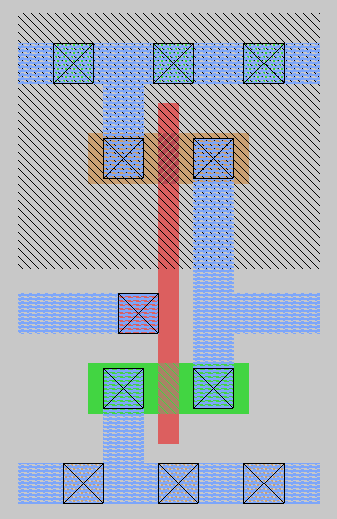
\includegraphics[scale=0.5]{images/inversor.png} % scale=0.5 (é 50%)
	\caption{Inversor 2} %legenda da figura
	\label{inversor-2} %rotulo da figura
\end{figure}

%____________________________________________________________________________

% Inserindo figuras lado a lado

\documentclass[a4paper, 12pt]{article} 
\usepackage[top=2cm, bottom=2cm, left=2.5cm, right=2.5cm]{geometry}
\usepackage[utf8]{inputenc}
\usepackage{amsmath, amsfonts, amssymb}
\usepackage{graphicx} %pacote para inserir figuras
\usepackage{float} %força posicionamento da figura - para usar: subtituir [htb] por[H]
\usepackage[brazil]{babel} %força latex a escrever figura e não figure
\usepackage{lipsum} %para inserir textos lorem ipsum
\usepackage{subfig}
%\usepackage{setspace}

\begin{document}

\section{Inserindo Figuras lado a lado}

\begin{figure}[!htb] %tenta colocar here, depois top, depois bottom
	\centering %centraliza
	\label{FiguraTotal} %rotulo da figura
	\subfloat[Subfigura 1 \label{subfigura-1}]{ 
		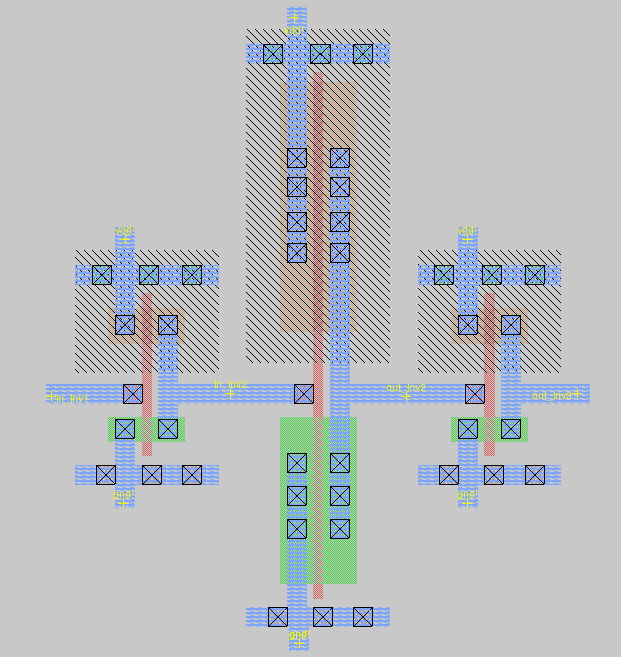
\includegraphics[width=0.48\textwidth]{images/inversores2.png} %width ou scale ou ...
	}\hfill
	\subfloat[Subfigura 2 \label{subfigura-2}]{ 
		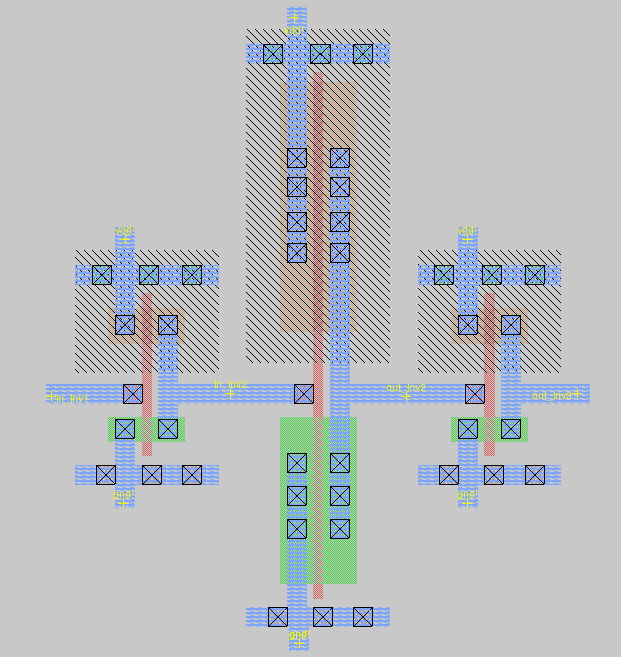
\includegraphics[width=0.48\textwidth]{images/inversores2.png}
	}
	\caption{Usando 2 figuras: \ref{subfigura-1} e \ref{subfigura-2} lado a lado com legenda} %legenda global das 2 figuras
\end{figure}


\end{document}


%____________________________________________________________________________


% Tabelas


\documentclass[a4paper, 12pt]{article} 
\usepackage[top=2cm, bottom=2cm, left=2.5cm, right=2.5cm]{geometry}
\usepackage[utf8]{inputenc}
\usepackage{amsmath, amsfonts, amssymb}
\usepackage{graphicx} %pacote para inserir figuras
\usepackage{float} %força posicionamento da figura - para usar: subtituir [htb] por[H]
\usepackage[brazil]{babel} %força latex a escrever figura e não figure
\usepackage{lipsum} %para inserir textos lorem ipsum


\begin{document}

\section{Veja uma tabela normal:}

\begin{table}[htb] %para colocar numerações na tabela
	\centering %centraliza a tabela :D
	\begin{tabular}{|c|c|} %indicamos o numero de colunas com alinhamentos lrc ou p{8cm} , |==borda
		\hline
		coluna 1 & coluna 2 \\ \hline %separamos linhas com barra barra
		coluna 1 & coluna 2 \\ \hline %hline é a linha horizontal
		coluna 1 & coluna 2 \\ \hline
	\end{tabular}
	\caption{tabela legenda numerada}	
	\label{index-tabela1}	%usar \ref{index-tabela1}} para referir-se à essa tabela
\end{table}

a tabela \ref{index-tabela1} é muito legal!


\section{Veja um cabeçalho para uma tabela:}

\begin{center}
	\begin{tabular}{cp{10cm}}
	\hline
		\begin{tabular}{c}
			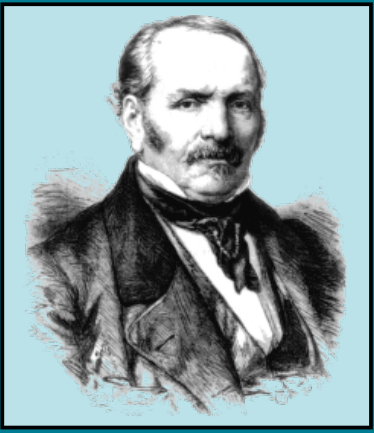
\includegraphics[scale=0.1]{img/kardec.png}				
		\end{tabular} & %aqui começa segunda coluna
		\begin{tabular}{l}
		latex é um negocio doido mano \\
		to aprendendo e curtindo \\
		legal \\
		
		\end{tabular}
	
	\end{tabular}
\end{center}
	

\end{document}





%____________________________________________________________________________

% Texto completo

\documentclass[a4paper, 12pt]{article} 
\usepackage[top=2cm, bottom=2cm, left=2.5cm, right=2.5cm]{geometry}
\usepackage[utf8]{inputenc}
\usepackage{amsmath, amsfonts, amssymb}
\usepackage{graphicx} %pacote para inserir figuras
\usepackage{float} %força posicionamento da figura - para usar: subtituir [htb] por[H]
\usepackage[brazil]{babel} %força latex a escrever figura e não figure
\usepackage{indentfirst} %identa o primeiro parágrafo após uma seção
\usepackage{lipsum}

\title{ \textbf{Título do trabalho}}
\author{Maurício Barbosa da Rocha \\ mauricio.mbr@gmail.com}
\date{2020}

\begin{document}

 \maketitle  %comando para escrever o título, pular página: \newpage

 \newpage	

 \tableofcontents \newpage %insere sumário
 
 \listoffigures \newpage %insere lista de figuras 
 
 \listoftables \newpage %insere lista de tabelas
 
%------------------------------------------------------------------- INTRODUÇÃO

 \section{Introdução}
  \lipsum[10] \lipsum[10]
  
 \begin{figure}[htb]
   \centering
   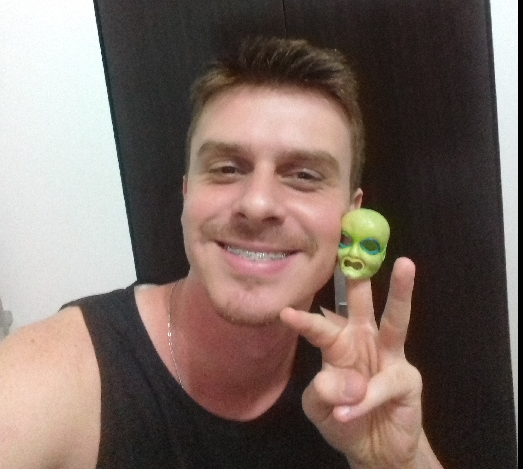
\includegraphics[scale=0.3]{imagens/eu1.png}
   \caption{Maurício e o et}
   \label{rotulo-figura1}
 \end{figure}

%------------------------------------------------------------------- DESENVOLVIMENTO  
 \section{Desenvolvimento}
  \lipsum[10]
  
 \subsection{Parte I do desenvolvimento}
 \lipsum[10]
  	 
 \subsubsection{Parte I - a do desenvolvimento}
 \lipsum[10]
  	   
 \begin{figure}[htb]
   \centering
   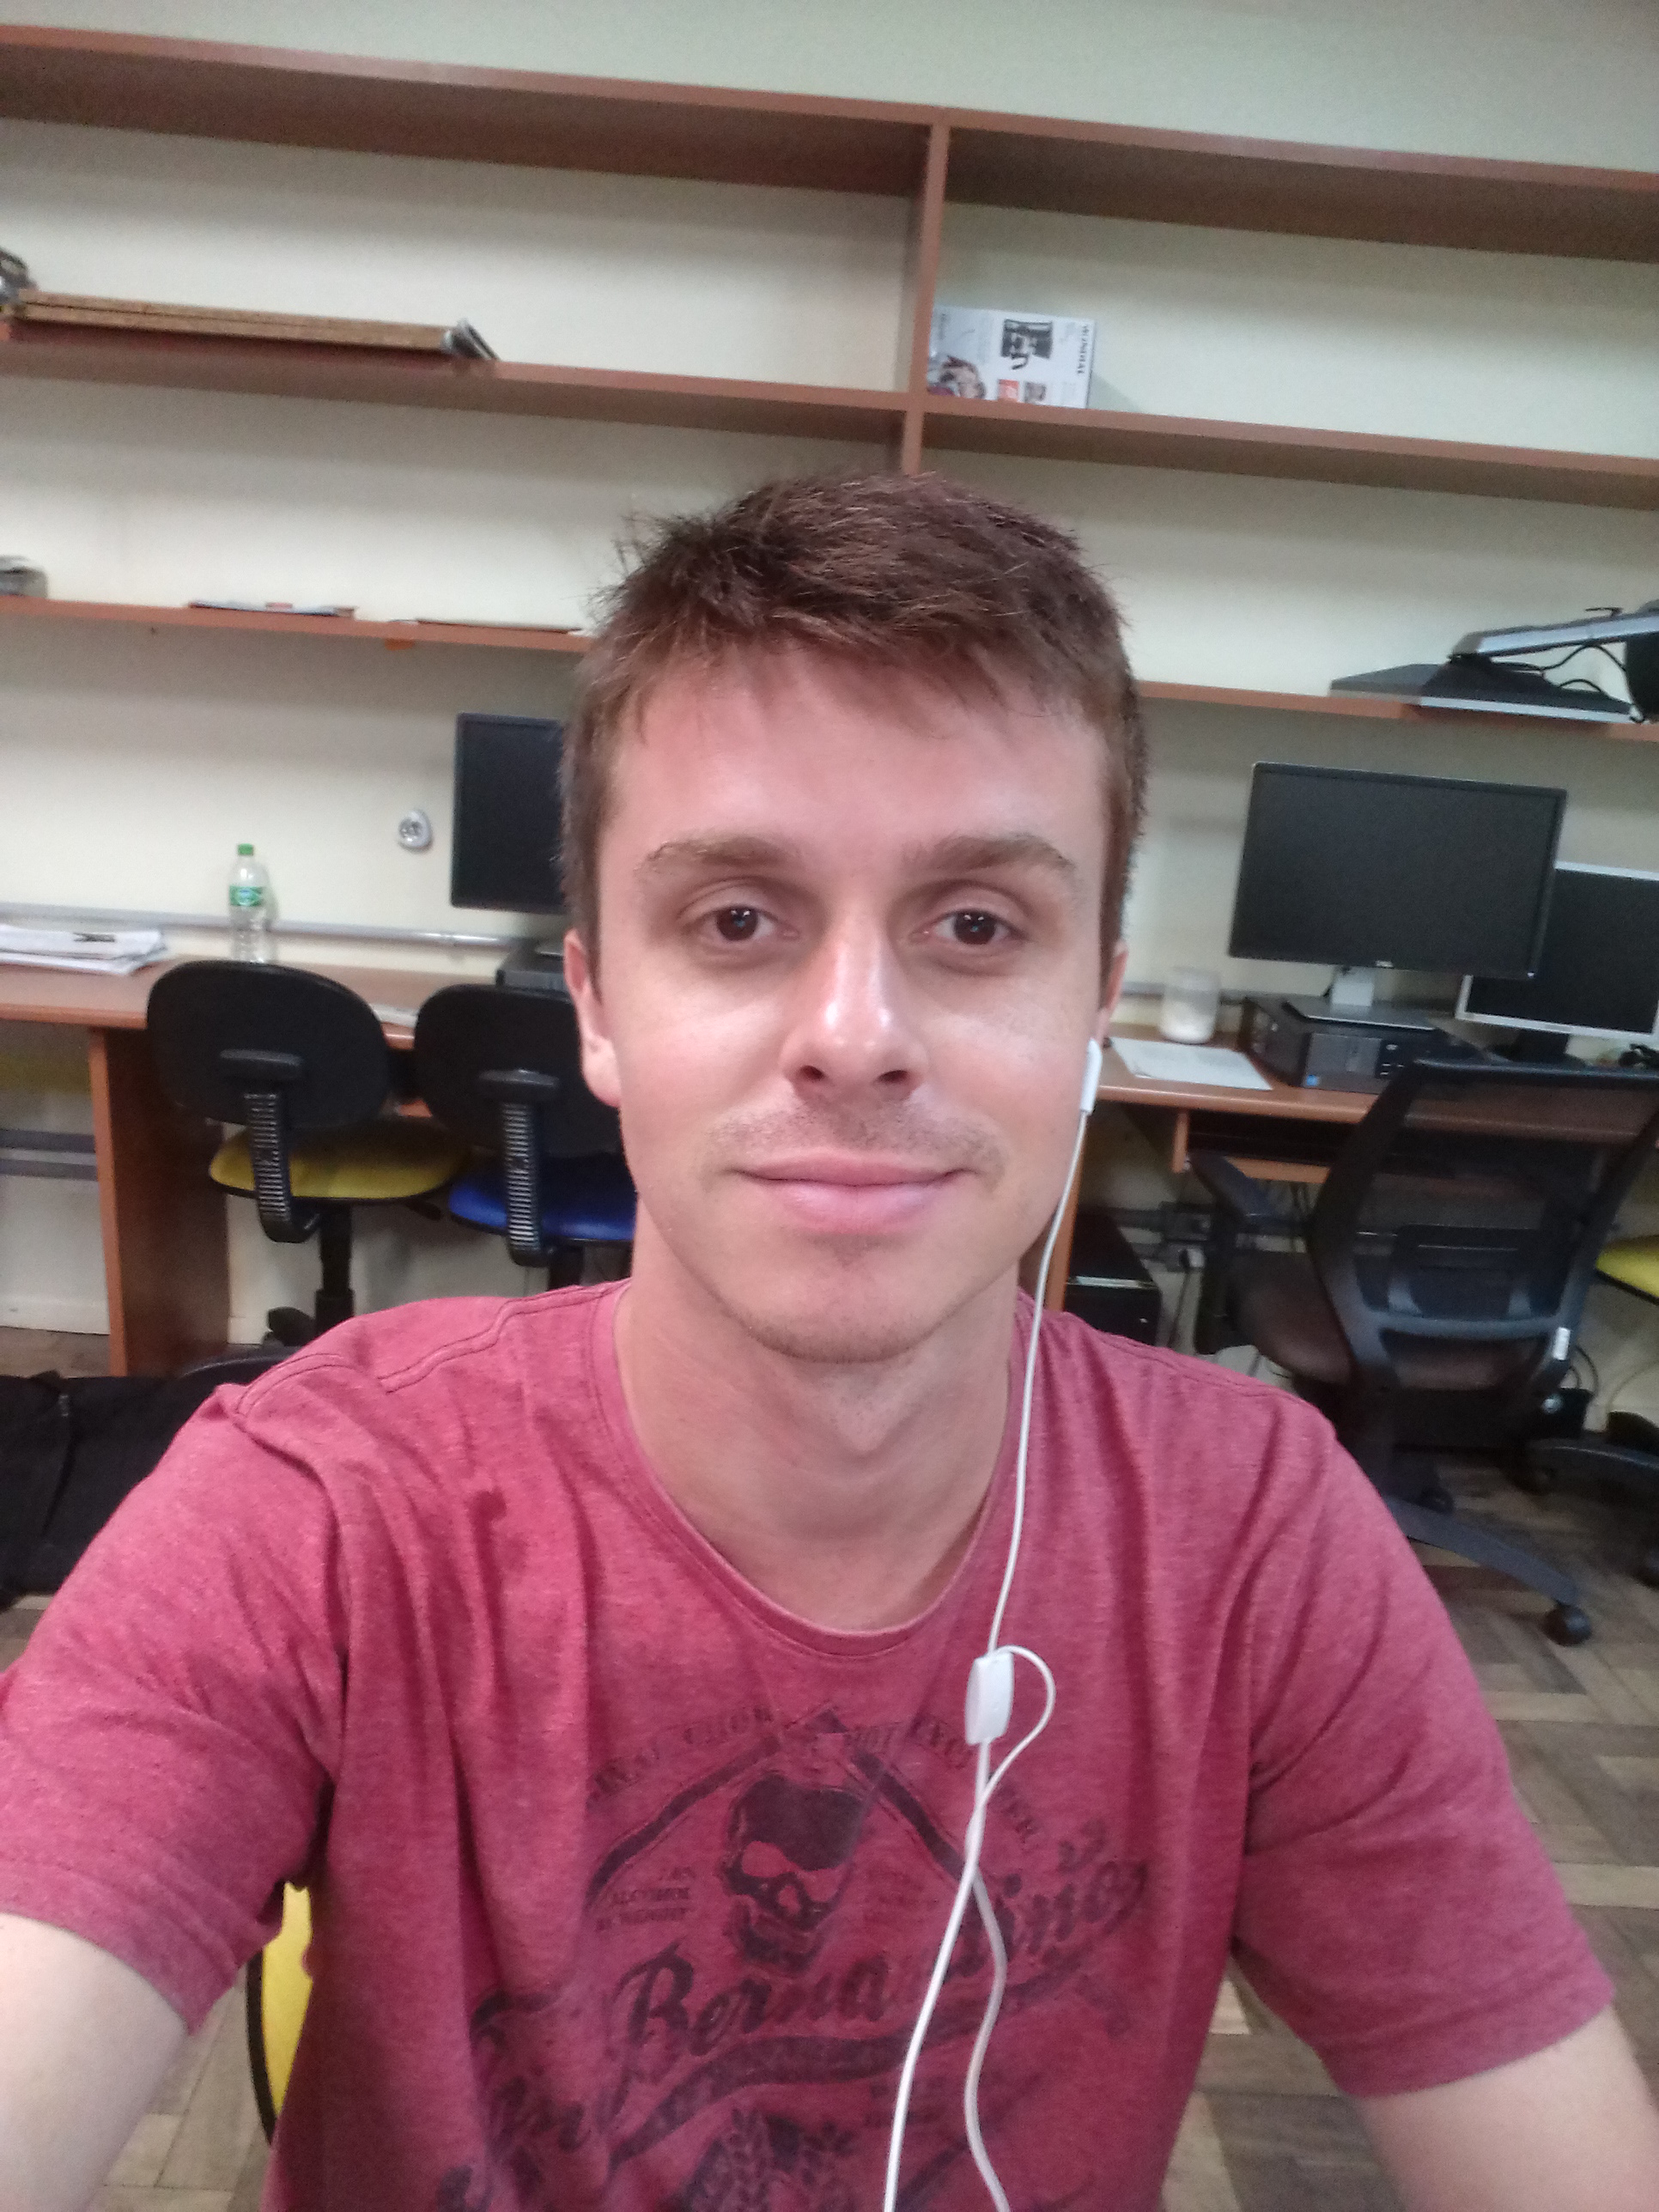
\includegraphics[scale=0.3]{imagens/eu2.jpg}
   \caption{Maurício no sensoriamento}
   \label{rotulo-figura2}
 \end{figure}
 
%------------------------------------------------------------------- CONSLUSÃO 
 \section{Conclusão}
 \lipsum[1]
 
 \begin{table}[htb]
   \centering
   \begin{tabular}{|c|c|}
     aaa1 & aaa2 \\
     aaa1 & aaa2 \\
   \end{tabular}
   \caption{Minha tabela 1}
   \label{minha-tabelinha}
 \end{table}
 
 Aqui estou citando um livro: \cite{meuatalho} 

 Aqui estou citando uma artigo: \cite{meuatalho2}
 

%------------------------------------------------------------------- REFERÊNCIAS BIBLIOGRÁFICAS
\newpage
\bibliographystyle{plain}
\addcontentsline{toc}{section}{Referências} %adiciona referencias ao sumário
\bibliography{referencia.bib} %nome do arquivo que contem as bibliografias Usar F11 para compilar

\end{document}


%__________________________

%%arquivo referencia.bib:

@book {meuatalho,
title="Título do Livro",
author="Autor do livro",
publisher="Editora do livro",
address="Cidade",
year="2010"
}

@article {meuatalho2,
title="Título do Artigo",
author="Autor do artigo",
journal="Revista do artigo",
year="2010"
}




%____________________________________________________________________________

% Inserindo links para o próprio documento


\documentclass[a4paper, 12pt]{article} 
\usepackage[top=2cm, bottom=2cm, left=2.5cm, right=2.5cm]{geometry}
\usepackage[utf8]{inputenc}
\usepackage{amsmath, amsfonts, amssymb}
\usepackage{graphicx} %pacote para inserir figuras
\usepackage{float} %força posicionamento da figura - para usar: subtituir [htb] por[H]
\usepackage[brazil]{babel} %força latex a escrever figura e não figure
\usepackage{indentfirst} %identa o primeiro parágrafo após uma seção
\usepackage{lipsum}

\begin{document}

\section{Nome da seção}
\lipsum[10]

\section*{Nome da seção} %seçao sem numeração - nao aparece nas referências
\lipsum[10]


\end{document}


%____________________________________________________________________________

Continuação: 


criar capa para o trabalho
começar a contar páginas após a capa
gerar links no sumário
mudar a forma de exibir a numeração das seções





%____________________________________________________________________________















